\section{Manuel Gómez Hernández}
\subsection{Definiciones}

\begin{enumerate} 
\item \textbf{La'tex: }
     \\Sistema de composición tipografica de alta calidad.

\item \textbf{GitHub: }
    \\Forja para alojar proyectos utilizando el sistema de control de git.

\item \textbf{git: }
    \\Sistema de control de versiones distrubuido, lo que significa que es un clon local de proyectos, es un repositorio de control de versiones completas.

\item \textbf{Precision: }
    \\Es la variación, disperción, poca variación, significa un buen grado de precisión.

\item \textbf{Exactitud: }
    \\Se define con respecto a su cercania (sesgo), mayor cercania implica un buen grado de exactitud.

\item \textbf{Estudio: } 
\begin{enumerate}
\item Esfuerzo que pone el entendimiento aplicándose a conocer algo.
\\ \textit{Análisis, investigación, observación, examen.}
\item Trabajo empleado en aprender y cultivar una ciencia o arte.
\\ \textit{Aprendizaje, formación, instrucción, preparación, enseñanza, aplicación, memorización.}
\cite{RAE}
\end{enumerate}

\item \textbf{Trabajo: }
\begin{enumerate}
    \item Acción y efecto de trabajar.
    \\ \textit{Labor, faena, brega, operación, curro, curre, currelo.}
    \item Ocupación retribuida.
    \\ \textit{Empleo, oficio, profesión, ocupación, cargo, puesto, plaza, función, chamba.}
    \item Cosa que es resultado de la actividad humana.
    \\ \cite{RAE}
\end{enumerate}

\item \textbf{Estudio de movimientos y tiempos: }
\\ Es el análisis de métodos, materiales, herramientas e instalación utilizada o que se ha de utilizar en la ejecución de un trabajo.
\\ \cite{DiapositivasSema-2-21}

\item \textbf{Análisis: }
\begin{enumerate}
    \item Distinción y separación de las partes de algo para conocer su composición.
    \\ \textit{Expliración, investigación, observación.}
    \item Estudio detallado de algo, especialmente de una obra o de un escrito.
    \\ \textit{Estudio, examen.}
    \\ \cite{RAE}
\end{enumerate}

\item \textbf{Sistema: }
\begin{enumerate}
    \item Conjunto de reglas o principios sobre una materia racionalmente enlazados entre sí.
    \\ \textit{Método, procedimiento, plan, manera, forma, modo, medio, técnica.}
    \item Conjunto de cosas que relacionadas entre sí ordenadamente contribuyen a determinado objeto.
    \\ \textit{Ordenación, organización, estructura, taxonomía.}
    \\ \cite{RAE}
\end{enumerate}

\item \textbf{Tiempo: }
\begin{enumerate}
    \item Duración de las cosas sujetas a mudanza.
    \\\textit{Duración.}
    \item Magnitud física que permite ordenar la secuencia de los sucesos, estableciendo un pasado, un presente y un futuro, y cuya unidad en el sistema internacional es el segundo.
    \item Parte de la secuencia de los sucesos.
    \\ \cite{RAE}
\end{enumerate}

\item \textbf{Predeterminar: }
\begin{enumerate}
    \item Determinar o resolver con anticipación algo.
    \\ \textit{Preestablecer, prefijar, estipular, preconcebir}
    \\ \cite{RAE}
\end{enumerate}

\item \textbf{Sistemas de tiempo predeterminado (STP): }
    \\ Conjunto de reglas o métodos para determinar con anticipación la secuencia de sucesos.
    \\ \cite{DiapositivasSema-2-21}

\item \textbf{Estudio de micromovimientos: }
    \\Division de la asignación de trabajo en therbligs que se logra mediante el analisis, cuadro por cuadro de una pelicula y la mejora de la operación a traves de la eliminación de los movimientos innecesarios y la simplificación de los necesarios.

\item \textbf{Estudio de metodos: }
    \\factores fundamentales en la determinación de la productividad de los operarios.

\item \textbf{MTM: }
    \\Métodos de medición del tiempo.
    \\Medición de tiempos de métodos.
    \\ \cite{DiapositivasSema-2-22}

\item \textbf{TMU: }
    \\Unidades de medida de tiempo.
    \\ \cite{DiapositivasSema-3-27}

\item \textbf{(1)Alcanzar (Reach "R"): }
    \\Por alcanzar se entiende el movimiento realizado con la mano vacía.
    \\ \cite{DiapositivasSema-3-27}

\item \textbf{(2)Mover (Move "M"): }
    \\Se refiere al movimiento con un objeto en la mano.
    \\ \cite{DiapositivasSema-3-27}

\item \textbf{FD: }
    \\Fáctor dinámico.
    \\ \cite{DiapositivasSema-3-27}

\item \textbf{CE-TMU: }
    \\Constante estática TMU.
    \\ \cite{DiapositivasSema-3-27}

\item \textbf{Muestreo: }
    \begin{enumerate}
        \item Acción de escoger muestras representativas de la caludad o condiciones meidias de un todo.
        \item Técnica empleada en un muestreo.
        \item Selección de una pequeña parte estadísticamente determinada, utilizada para inferir el valor de una o varias características del conjunto.
        \\ \textit{Unidad de muestreo.}
        \\ \cite{DiapositivasSema-4-04}
    \end{enumerate}

\item \textbf{Representativo, va: }
\begin{enumerate}
    \item Que sirve para representar algo.
    \\ \textit{Característico, propio, peculiar, específico, clásico, típico, individual.}
    \item Que representa con justos títulos.
    \\ \textit{Relevante, significativo, importante.}
    \\ \cite{RAE}
\end{enumerate}

\item \textbf{Infeir: }
\begin{enumerate}
    \item Deducir algo o sacarlo como conclusión de otra cosa.
    \\\textit{Deducir, derivar, concluir, colegir, inducir.}
    \item Producir un daño físico o moral.
    \\ \textit{Infligir, dañar, lastimar, herir.}
    \item Incluir o llevar consigo algo.
    \\ \cite{RAE}
\end{enumerate}

\item \textbf{Muestreo: }
    \\Acción de escoger muestras que describan de manera exacta las características de un conjunto de datos que permitirán deducir y sacar conclusiones del fenómeno a estudiar.
    \\ \cite{DiapositivasSema-4-04}

\item \textbf{Muestro del trabajo: }
    \\Herramienta para disminuir el costo que se presenta en el estudio continuo del tiempo.
    \\ \cite{DiapositivasSema-4-04}

\item \textbf{Muestreo discreto: }
    \\Implica seleccionar elementos específicos de una población finita o contable, donde cada elemento tiene una probabilidad asociada de ser elegido.
    
\item \textbf{Muestreo continuo: }
    \\Selección de elementos de una población infinita, donde los valores pueden tomar cualquier valor dentro de un rango específico, como la altura o el tiempo.

\item \textbf{Estudio de tiempos convencional: }
    \\Es una muestra continua de n ciclos (Suponiendo que la distribución estadística es normal).
    \\ \cite{DiapositivasSema-4-04}

\item \textbf{Distribución estadística normal: }
    \\Forma de distribución estadística simétrica con forma de campana, donde la mayoría de los datos se concentran cerca de la media.

\item \textbf{Estudio de tiempos no convencional: }
    \\Es una muestra discreta (Suponiendo que la distribución estadística es binomial).
    \\ \cite{DiapositivasSema-4-04}

\item \textbf{Distribución estadística binomial: }
    \\Modelo estadístico que describe la probabilidad de obtener un número específico de éxitos en un número fijo de ensayos independientes, donde cada ensayo tiene dos resultados posibles: éxito o fracaso.

\item \textbf{Pronostico: }
    \\Valor que se cree obtener.
    
\item \textbf{Estimación: }
    \\Analisis a traves de operaciones.

\end{enumerate}

\subsection{Materiales}


\subsubsection{Tabla de materiales}

\subsubsection{Trazado de Materiales }

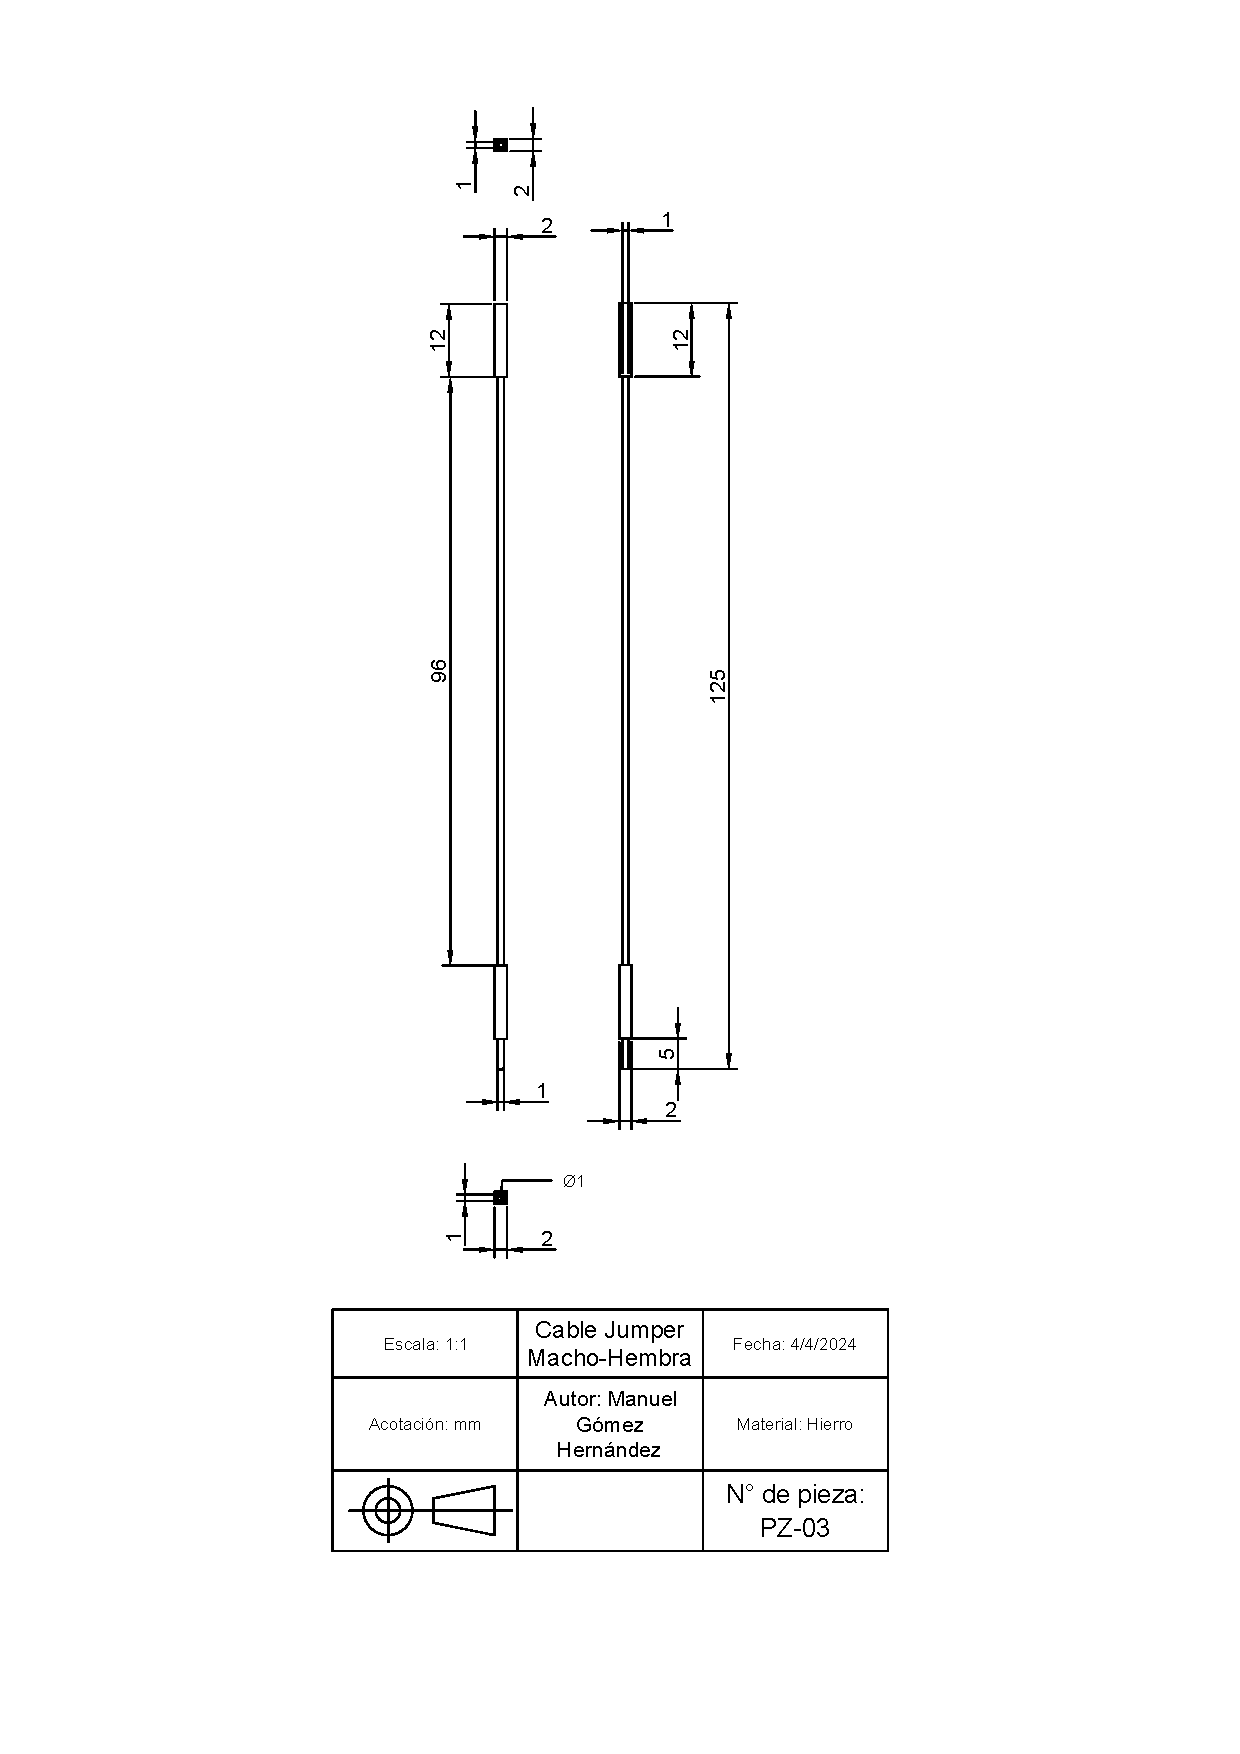
\includegraphics[width=.9\textwidth]{15/img/cableJumperMHTrazo.pdf}~\\[15cm]
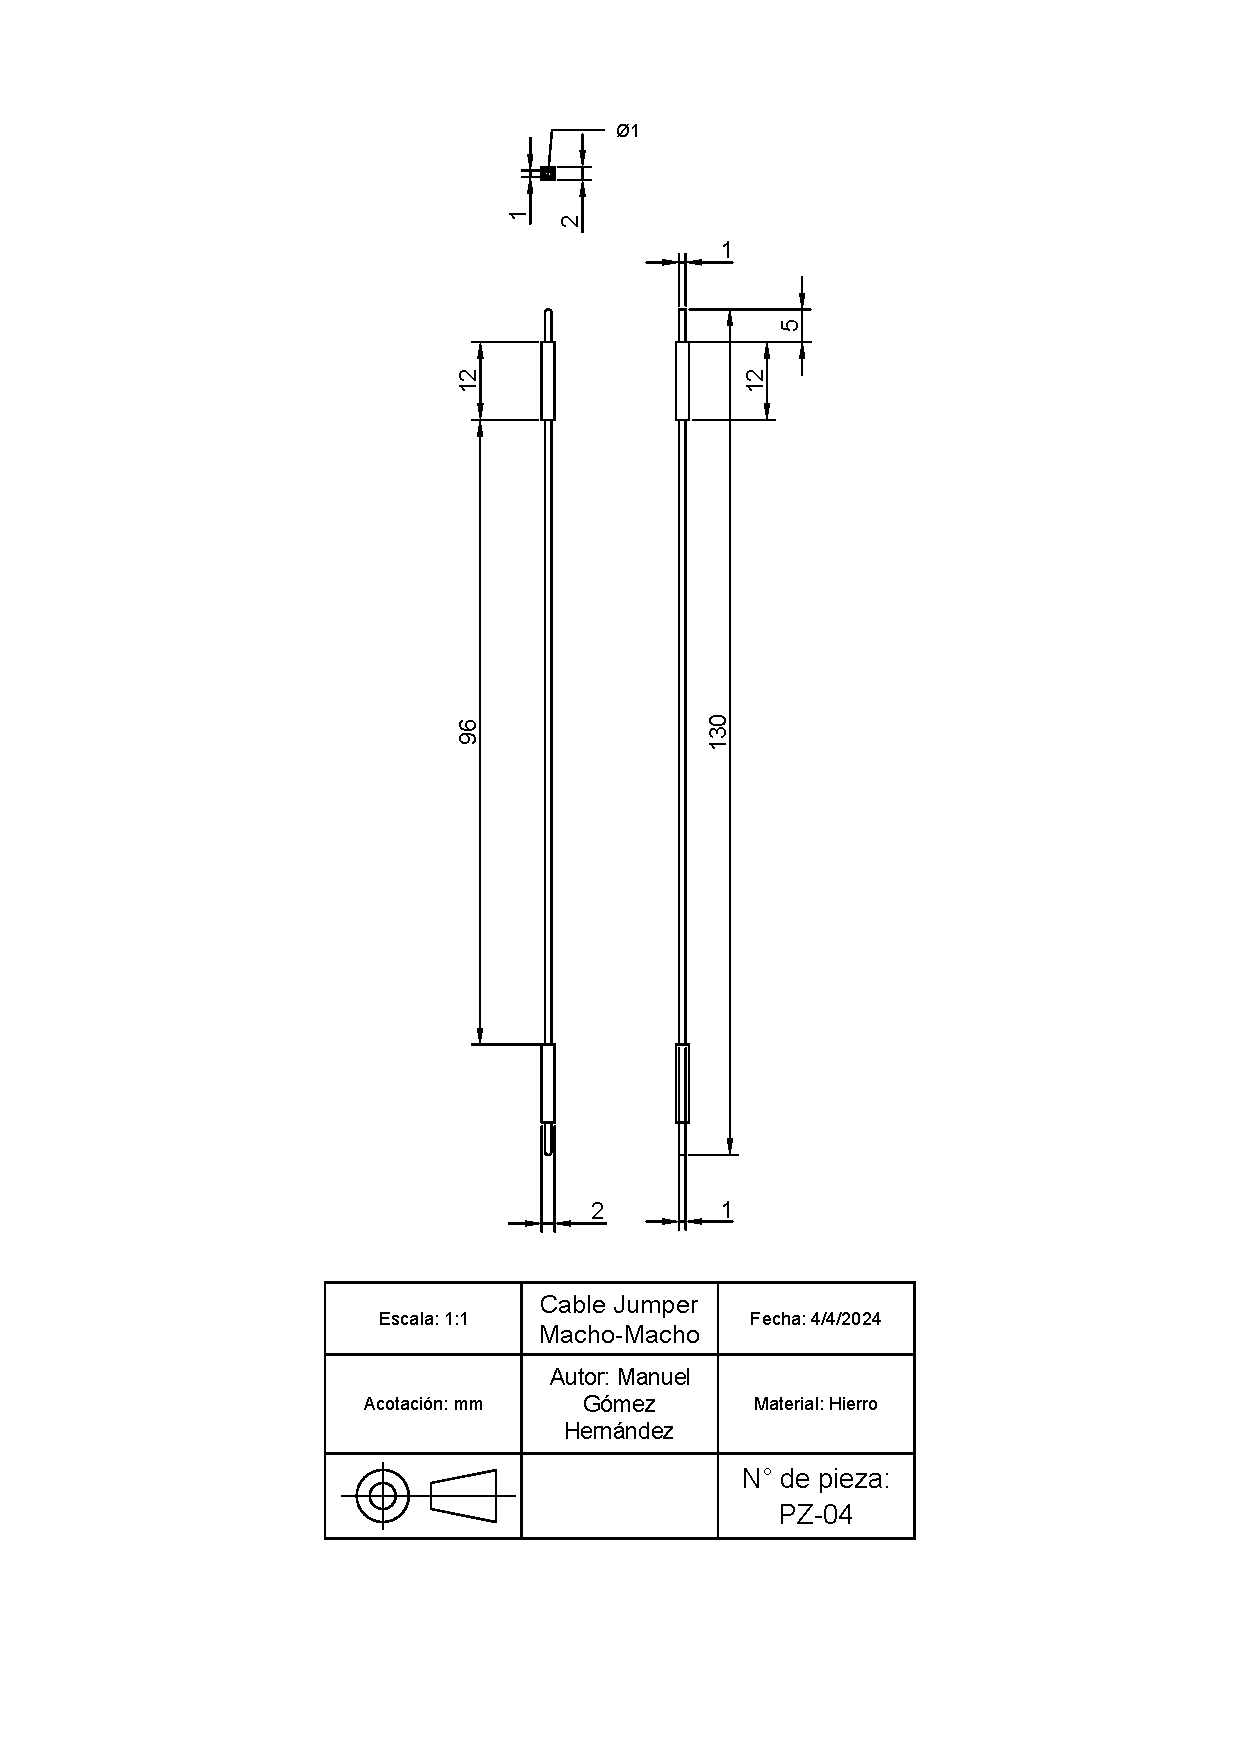
\includegraphics[width=.9\textwidth]{15/img/cableJumperMMTrazo.pdf}~\\[15cm]
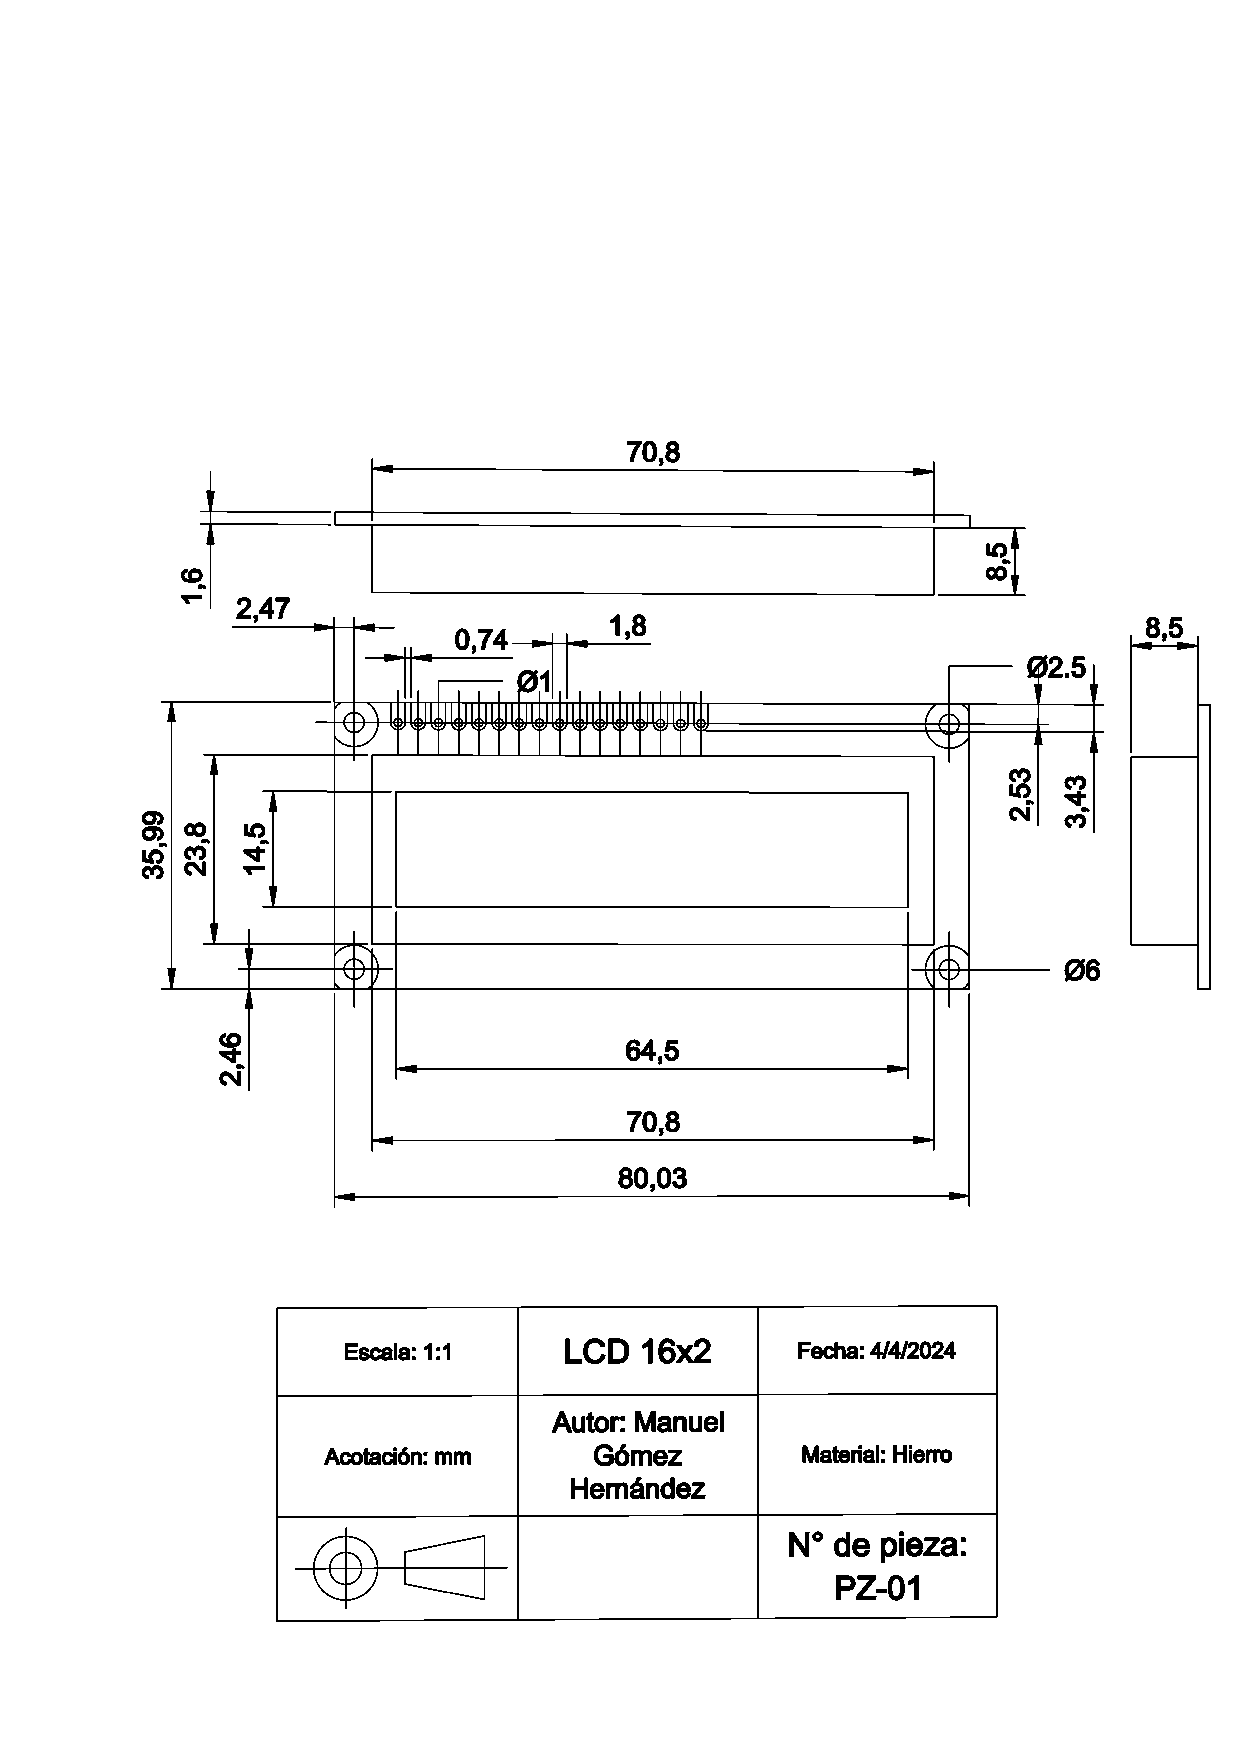
\includegraphics[width=.9\textwidth]{15/img/lcdTrazo.pdf}~\\[15cm]
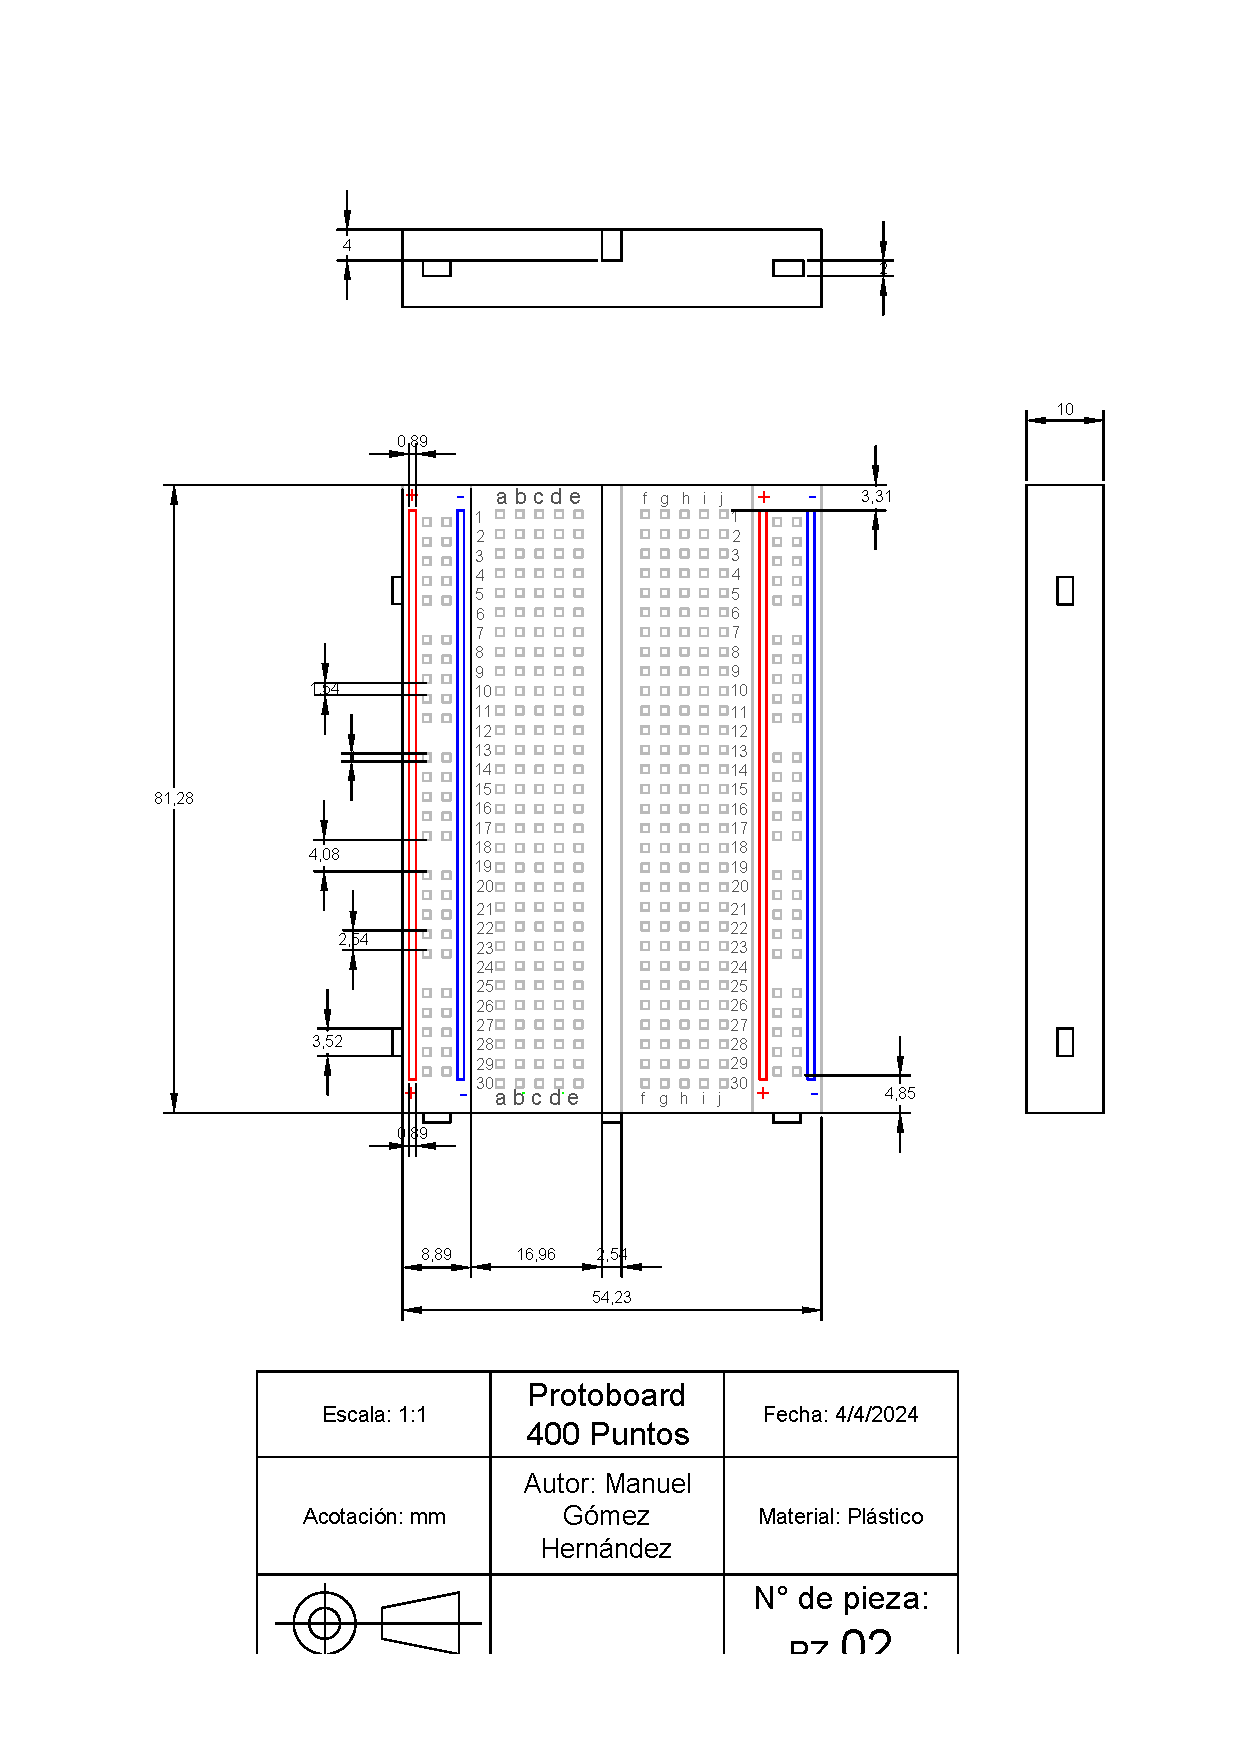
\includegraphics[width=.9\textwidth]{15/img/placaProtoboardTrazo.pdf}~\\[15cm]
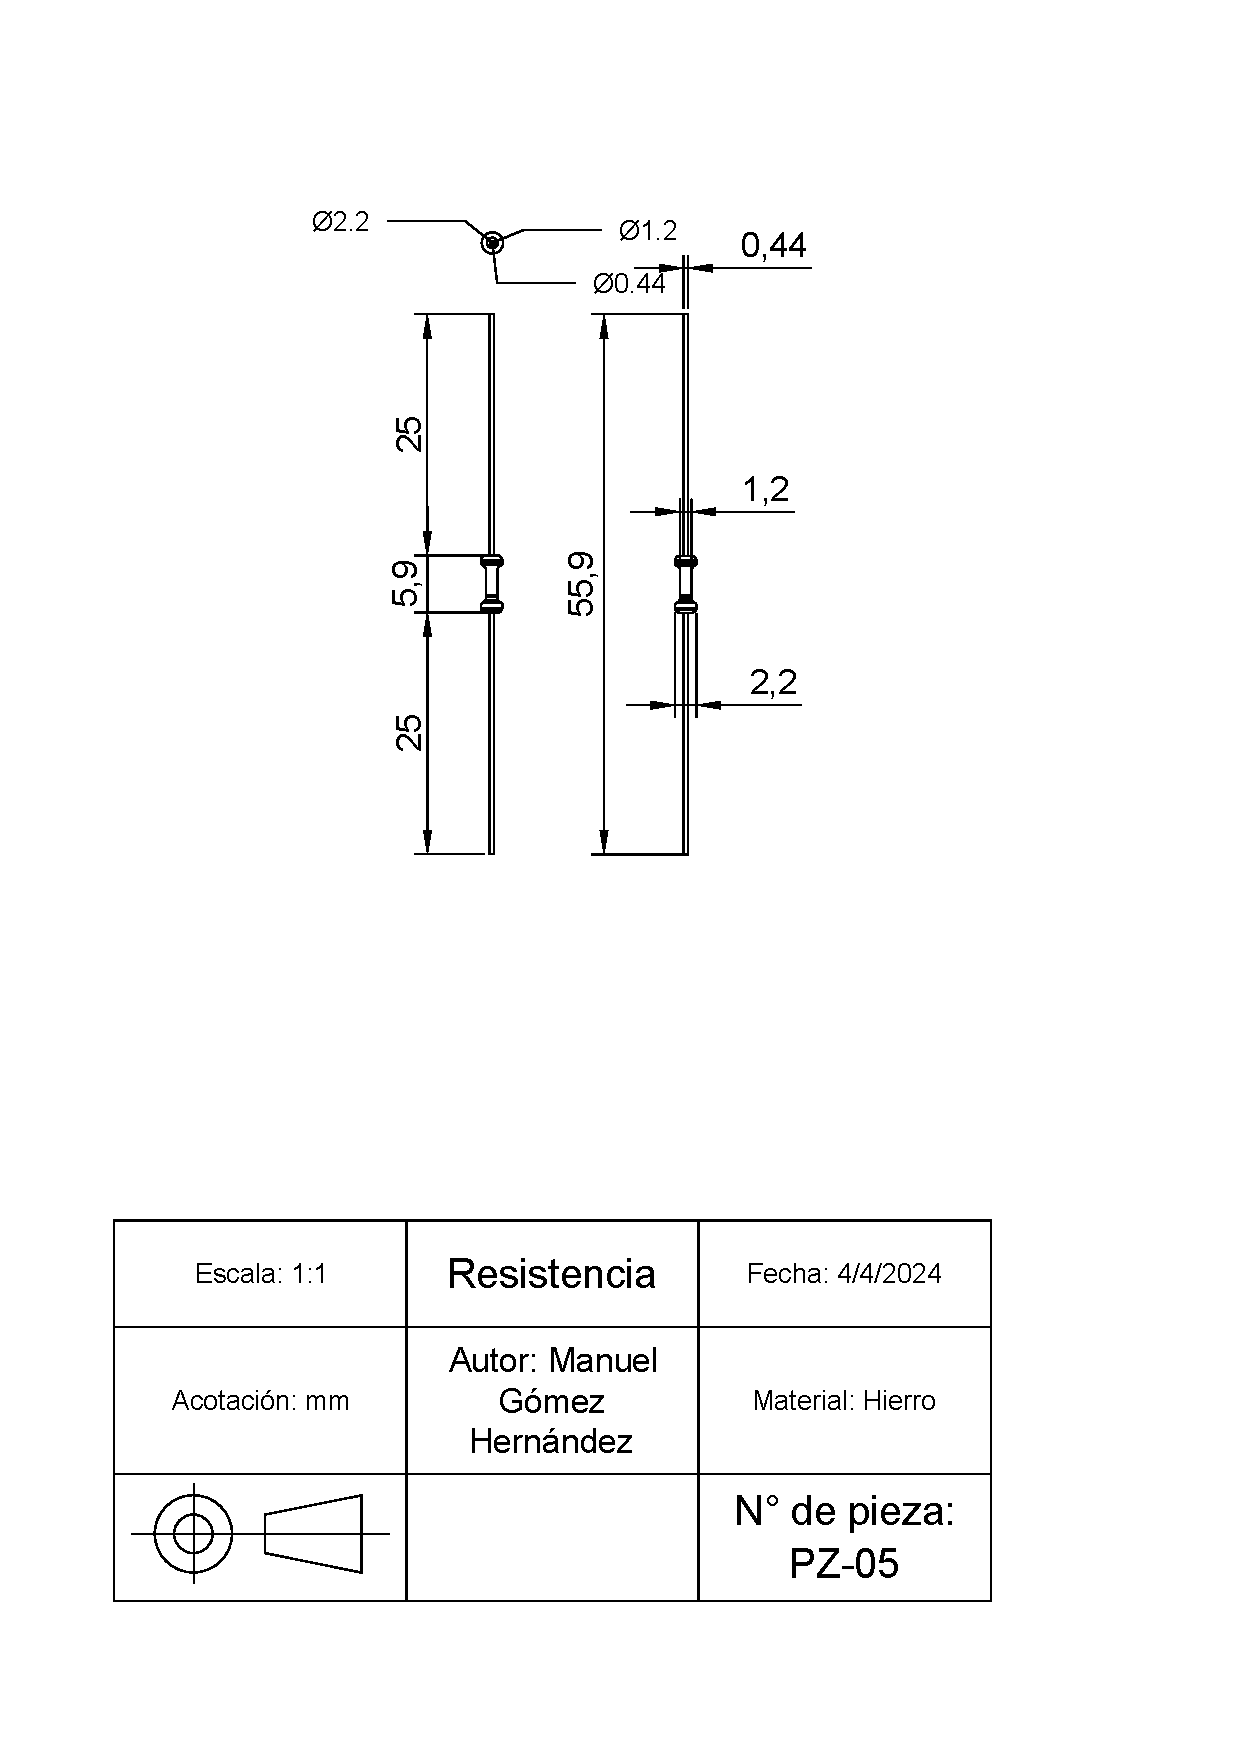
\includegraphics[width=.9\textwidth]{15/img/resistenciaTrazo.pdf}~\\[15cm]



\lhead{\begin{tikzpicture}[remember picture, overlay]
    \node [anchor=100,inner sep=0] (imagenIZQUIERDA) at (current page header area.north){
\includegraphics[width=18cm]{img/Encabezado.PNG}};
    \end{tikzpicture}}
    \rhead{Gómez-Hernández}
    \rfoot{\begin{tikzpicture}[remember picture, overlay]
    \node [anchor=140,inner sep=0] (imagenDERECHA) at (current page footer area.south){
\includegraphics[width=18cm]{img/Foot.PNG}};
    \end{tikzpicture}}
    %----------------------------------------------------------------------------------------
    \lfoot{ \thepage}
    % \renewcommand{\labelenumi}{\alph{enumi}.)} 
    %----------------------------------------------------------------------------------------
    %----------------------------------------------------------------------------------------
    %	TITLE SECTION
    %----------------------------------------------------------------------------------------
    
    \setlength{\droptitle}{-5\baselineskip} % Move the title up
    \title{\textbf{Estudio de tiempos y movimientos en el ensamble de un circuito electrónico utilizando diferentes métodos para su optimización }} % Article title
    
     \author{ 
     \textsc{Gómez-Hernández, Manuel}\\ 
    %  Afiliación:
     \texttt{Instituto Tecnológico de Querétaro } \\ 
     \texttt{Tecnológico Nacional de México} \\ 
     \texttt{Querétaro, México}\\ 
     \texttt{Correo} 
     \and 
     \textsc{Ángeles-Hurtado, Luis Alberto}\\ 
    %  Afiliación:
     \texttt{ Instituto Tecnológico de Querétaro } \\ 
     \texttt{ Tecnológico Nacional de México } \\ 
     \texttt{Querétaro, México}\\ 
     \texttt{alb3rt0.ah@gmail.com} 
    }
    
    
    %----------------------------------------------------------------------------------------
    
    % \begin{document}
    
    % Print the title
    \maketitle
    \thispagestyle{fancy}
    
    %----------------------------------------------------------------------------------------
    %	ARTICLE CONTENTS
    %----------------------------------------------------------------------------------------
    
    % \section*{Resumen}
    % \textit{Palabras clave:}
    % El resumen (ancho de página) deberá contener entre 100 y 200 palabras tipo Adobe Devangari 11 puntos.
    
    \begin{abstract}
    \noindent 
    El resumen (ancho de página) deberá contener entre 100 y 200 palabras tipo Adobe Devangari 11 puntos.
    
    \end{abstract}
    % 
    % 
    \textbf{\textit{Palabras clave}}: {First keyword should be the corresponding to the research area according with the authors guide. Maximum of 6 keywords.}
    % \keywords{First keyword should be the corresponding to the research area according with the authors guide. Maximum of 6 keywords.}
    
    \section{Introducción}
    
    % Define estudio de tiempos y movimientos
    % define que es ensamble
    % define que es circuito electronico
    % define el metodo de tiempos predeterminados
    % define optimización
    \begin{itemize}
        \item 
    El Estudio de Tiempos y Movimientos es una técnica fundamental en la gestión de la eficiencia empresarial, que fusiona dos importantes contribuciones al campo de la administración industrial. Por un lado, el Estudio de Tiempos, desarrollado por Frederick Winslow Taylor, se centra en la medición y análisis del tiempo necesario para llevar a cabo una tarea específica. Por otro lado, el Estudio de Movimientos, creado por Frank y Lillian Gilbreth, se enfoca en analizar y mejorar los movimientos físicos realizados por los trabajadores durante la ejecución de dicha tarea. En el cual se emplean diversas metodologias como MTM: Descompone tareas y asigna tiempos estándar, MTD: Se centra en desarrollar métodos de trabajo eficientes, MOST: Analiza la secuencia de operaciones necesarias, MODAPTS: Utiliza elementos de tiempo predeterminados, BMT: Asigna tiempos estándar a movimientos básicos. Estas metodologías ayudan a mejorar la eficiencia en los procesos industriales. 
    
    En este proyecto, nos enfocaremos en la creación de un sistema de control electrónico que empleará diversos materiales indespensables como un controlador ESP32, un potenciómetro y una pantalla LCD de 16x2, por mencionar los mas sobresalientes, cuales nos brindaran la información requerida. [1]
    
    \end{itemize}
    % 
    % 
    \section{Justificación}
    
    \begin{itemize}
        \item El objetivo principal del proyecto actual es revisar y optimizar los sistemas utilizados en su elaboración, utilizando tecnologías avanzadas y metodologias  para mejorar la eficiencia y evaluar el rendimiento. Emplearemos el estudio de tiempos y movimientos haciendo mejoras continuas y obteniendo la mayor eficiencia.[1]
    \end{itemize}
    % 
    % 
    \section{Descripción del problema}
    \begin{itemize}
        \item Optimizar el procedimiento para el ensamble de un circuito electrónico, buscando el resultado mas efectivo, eliminando los movimientos inecesarios asi como mejorando los necesarios y aplicando diversas tecnicas de mejora, haciendo mas sencillas las tareas del operador y del analista.
    \end{itemize}
    
    \textbf{*La incógnita científica es el elemento cuya solución incrementa el conocimiento científico.}
    % 
    % 
    \section{Fundamentación teórica}
    
    Es la parte medular y de mayor discusión, deberá ser la fundamentación de la hipótesis, por tanto se deberá señalar claramente la razón de la suposición y fundamentación de la misma. Únicamente referencias científicas.
    \begin{itemize}
        \item Se debe de retomar el tema que se planteo en la introducción, pero ahora profundizando para clarificar la incógnita científica y se pueda plantear la hipótesis.
        \item Se debe de retomar la descripción del problema, pero ahora a profundidad del (los) objeto(s) de estudio. 
        \item Se debe de profundizar en las metodologías que se ha usado para el estudio del tema.
        \item Referencias solo de artículos y libros científicos.
    \end{itemize}
    % 
    % 
    \section{Hipótesis}
    
    Es la suposición con fundamento científico relativa a la solución del problema, necesidad o de cómo se aprovecha la oportunidad con la incógnita científica y se fundamenta con: 1. Una suposición (en afirmativo o negativo) y ésta deberá vincularse con:
    2. La fundamentación científica que deberá ser precisa 3. Una entidad de comparación para probar la suposición y
    4. La variable con que se califica o cuantifica la comparación o se prueba la hipótesis.
    
    \begin{itemize}
        \item Se debe de identificar claramente la suposición científica
        \item Se debe de identificar claramente el fundamento científico
        \item Se debe identificar claramente la variable de respuesta
        \item Se debe identifican claramente las realidades o modelos contrastantes
        \item Se debe de establecer las variables asociadas, explicativas o que tienen relación funcional con la variable de respuesta
    \end{itemize}
    % 
    % 
    \section{Objetivo}
    
    Precisar la acción necesaria para probar la hipótesis. Dicha acción se establece mediante el uso de verbos activos y en infinitivo.
    \begin{itemize}
        \item Se debe establecer que se pretende probar la hipótesis
    \end{itemize}
    
    \subsection{Objetivos específicos }
    
    \begin{itemize}
        \item Se debe establecer como un conjunto de acciones comunes para lograr el objetivo general
        \item Se debe establecer como etapas para lograr el objetivo general
    \end{itemize}
    
    Son actividades orientadas al cumplimiento del objetivo general. Se establecen con verbos activos en infinitivo. Son parte de la acción encaminada a probar la hipótesis. Éstos deben ser precisos, y en lo posible evitar aspectos metodológicos.
    % 
    % 
    \section{Cuerpo (Metodología, modelo matemático, etc.)}
    
    \begin{itemize}
        \item Lista de Materiales 
        \ref{anexo:listaDeMateriales.pdf}
    \end{itemize}

    \begin{itemize}
        \item Para el ensamblado de ESP-32-C6 y lograr la finalidad del proyecto utiliza el siguiente manual.
        \ref{anexo:manualDeEnsambleDeCircuitoElectronicoEsp32-c6.pdf}
    \end{itemize}


\subsection{Prepara tu documento}

    Antes de que comiences a utilizar esta plantilla, es recomendable que prepare la información que contendrá en un archivo aparte. 
    Ten preparadas tus gráficas, así como también las tablas aparte, para que sea más fácil integrarlo. 
    Se recomienda fuertemente el uso de \textbf{formato Enhanced Metafile (.emf) para imágenes y gráficas} de resolución óptima. 
    Finalmente, completa y organiza el contenido antes de darle el formato de esta plantilla. 

    
    \subsection{Acrónimos y Abreviaciones}
    
    Los acrónimos y abreviaciones deberán ser definidos únicamente la primera vez que aparecen en el texto, esto para que el lector entienda lo que significan.
    
    \subsection{Ecuaciones}
    
    Las ecuaciones son una excepción a las especificaciones prescritas de esta plantilla. 
    Deberá determinar si su ecuación debe escribirse o no utilizando la fuente Adobe Devangari. 
    Para crear ecuaciones multinivel, puede ser necesario tratar la ecuación como un gráfico e insertarla en el texto después de aplicar el estilo de la platilla.
    Las ecuaciones serán enumeradas de manera consecutiva, y el número de ecuación, entre paréntesis, se colocan al ras de la derecha, utilizando una tabulación derecha. 
    
    \begin{equation}
        \label{eq1}
        x + y = z 
    \end{equation}
    
    Es importante asegurarse de que los símbolos de la ecuación sean definidos antes o inmediatamente después de la ecuación. Utilice “(1)”, en vez de “Eq. 1” al enumerar las ecuaciones, excepto al principio de una oración: “La ecuación (\ref{eq1}) es…”
    
    \section{Resultados y discusión}
    
    Antes de comenzar a preparar tu artículo, es importante que lea primero la guía del autor, la cual incluye los temas o apartados que son necesarios para tener tu trabajo completo.
    Una vez completada la edición del texto, el documento está listo para el uso de esta plantilla. En este archivo recién creado, resalte todo el contenido e importe el archivo de texto preparado. Ahora esta listo para estilizar su documento.
    En esta sección se deben presentar todo lo obtenido de la sección 2, incluidas deducciones o efectos del desarrollo. También se podrán incluir subsecciones numeradas de la siguiente forma:
    
    \subsection{Autores y Afiliaciones}
    
    Para distinguir las afiliaciones de los autores, utilice superíndices iniciando con el número 1, 2, etc., sucesivamente, esto dependerá de la cantidad de los departamentos a los que estén afiliados los autores. En caso de que todos los autores pertenezcan a una mismo departamento e institución, utilizar sólo el superíndice 1. 
    
    \subsection{Identificar los encabezados}
    
    Se les recuerda a los autores que los encabezados deben de estar conforme los solicita la guía del autor. De ahí se puede adaptar el trabajo para que sea más fácil de entender para el lector.
    Los encabezados organizan los temas sobre una base relacional y jerárquica. Por ejemplo, el título del documento es encabezado del texto principal porque todo el material posterior se relaciona y elabora sobre este tema. 
    
    \subsection{Tablas y Figuras}
    
    \begin{enumerate}
        \item Posición de las tablas y figuras: Coloque las figuras y las tablas en la parte superior e inferior de las columnas. Evite colocarlos en medio. Las figuras y las tablas grandes pueden abarcar ambas columnas. Los títulos de las figuras deben de estar debajo de las mismas; los títulos de las tablas deben aparecer encima de ellas. Insértese las figuras y los cuadros después de citarse en el texto. Utilice la abreviatura “Fig. 1”, incluso al principio de una oración. 
    \end{enumerate}
    
    \section{Conclusiones}
    
    Se describe aquí el alcance del trabajo, logros obtenidos y perspectivas para el futuro de este. Se sugiere colocar información cuantitativa obtenida.
    
    \section{Agradecimientos}
    
    Es importante darles su debido reconocimiento a los laboratorios, instituciones, organizaciones, entre otros que han sido participes para la culminación de este trabajo. También es importante mencionar, fondos, proyectos, becas, entre otros que se le han otorgado al o los autores para realizar el trabajo de investigación. Ejemplo: “Los autores agradecen al Concejo Nacional de Ciencia y Tecnología por los recursos otorgados…”
    
    \section*{Referencias}
    
    [1] \cite{Maynard's}
    
    
    
    Para esta platilla, se solicita al autor enumerar las citas de manera consecutiva entre corchetes \cite{YLi2013}. 
    La puntuación de la oración que sigues sería \cite{Mesaelides2011}. 
    Refiérase simplemente al número de referencia, como en \cite{Morales2012}, no utilice “Ref. [3]” o “referencia [3]” excepto al principio de una oración: “La referencia [3] fue la primera…”
    Enumere las notas al pie por separado en superíndices. Coloque la nota de pie de en la parte inferior de la columna en la que se citó. No coloque notas al pie en la lista de referencias. Utilice letras para las notas al pie de la tabla.
    A menos de que haya tres autores o más; no utilice “et al.”. Los trabajos que no hayan sido publicados, incluso si han sido presentados para su publicación, deben ser citados como “inéditos”. Los trabajos que han sido aceptados para su publicación deben de citarse como “en prensa”. Poner en mayúscula sólo la primera palabra de un título, excepto los nombres propios y los símbolos de elemento. 
    Otros ejemplos \cite{LAAngeles2021}, \cite{LAAngelesConni}. 
    Véase el link \cite{prueba}.
    
    % Ejemplo
    %  @Article{article,
    % 	author = "Author1 LastName1 and Author2 LastName2 and Author3 LastName3",
    % 	title = "Article Title",
    % 	volume = "30",
    % 	number = "30",
    % 	pages = "10127-10134",
    % 	year = "2013",
    % 	doi = "10.3389/fnins.2013.12345",
    % 	URL = "http://www.frontiersin.org/Journal/10.3389/fnins.2013.12345/abstract",
    % 	journal = "Frontiers in Neuroscience"
    % }
    
    % @book{book,
    %   author    = {Author Name}, 
    %   title     = {The title of the work},
    %   publisher = {The name of the publisher},
    %   address   = {The city},
    %   year      = 1993,
    % }
    
    % @incollection{chapter,
    %   author       = {Bauthor Surname}, 
    %   title        = {The title of the work},
    %   editor       = {Editor Name},
    %   booktitle    = {The title of the book},
    %   publisher    = {The name of the publisher},
    %   address      = {The city},
    %   year         = 2002,
    %   pages        = {201-213},
    % }
    
    % @InProceedings{conference,
    %   author = {Cauthor Name and Dauthor Surname and Fauthor LastName},
    %   title = {The title of the work},
    %   booktitle = {The title of the conference proceedings},
    %   year = 1996,
    %   publisher = {The name of the publisher},
    %   editor = {Editor Name1 and Editor Name2},
    %   pages = {41-50},
    % }
    
    % @book{cho,
    %   author       = {Gauthor Name1}, 
    %   title        = {The title of the work},
    %   publisher = {Country code and patent number},
    %   address      = {Patent Country},
    %   year = 2013
    % }
    
    % @book{patent,
    %   author    = {Hauthor Surname1}, 
    %   title     = {The title of the work},
    %   publisher = {Patent number},
    %   address   = {Patent country},
    %   year      = 2010,
    % }
    
    % % please use misc for datasets
    % @misc{dataset, 
    % 	author = "Author1 LastName1 and Author2 LastName2 and Author3 LastName3",
    % 	title = "Data Title",
    % 	year = "2011",
    % 	doi = "10.000/55555",
    % 	URL = "http://www.frontiersin.org/",
    % }
    
    

    % 
    % 
    %%%%%%%%%%%%%%%%%%%%%%%%%%%%%%%%%%
    \appendix
    %%%%%%%%%%%%%%%%%%%%%%%%%%%%%%%%%%
    % 
    % 
    \centering{\section[\appendixautorefname{}]{APÉNDICE}}
    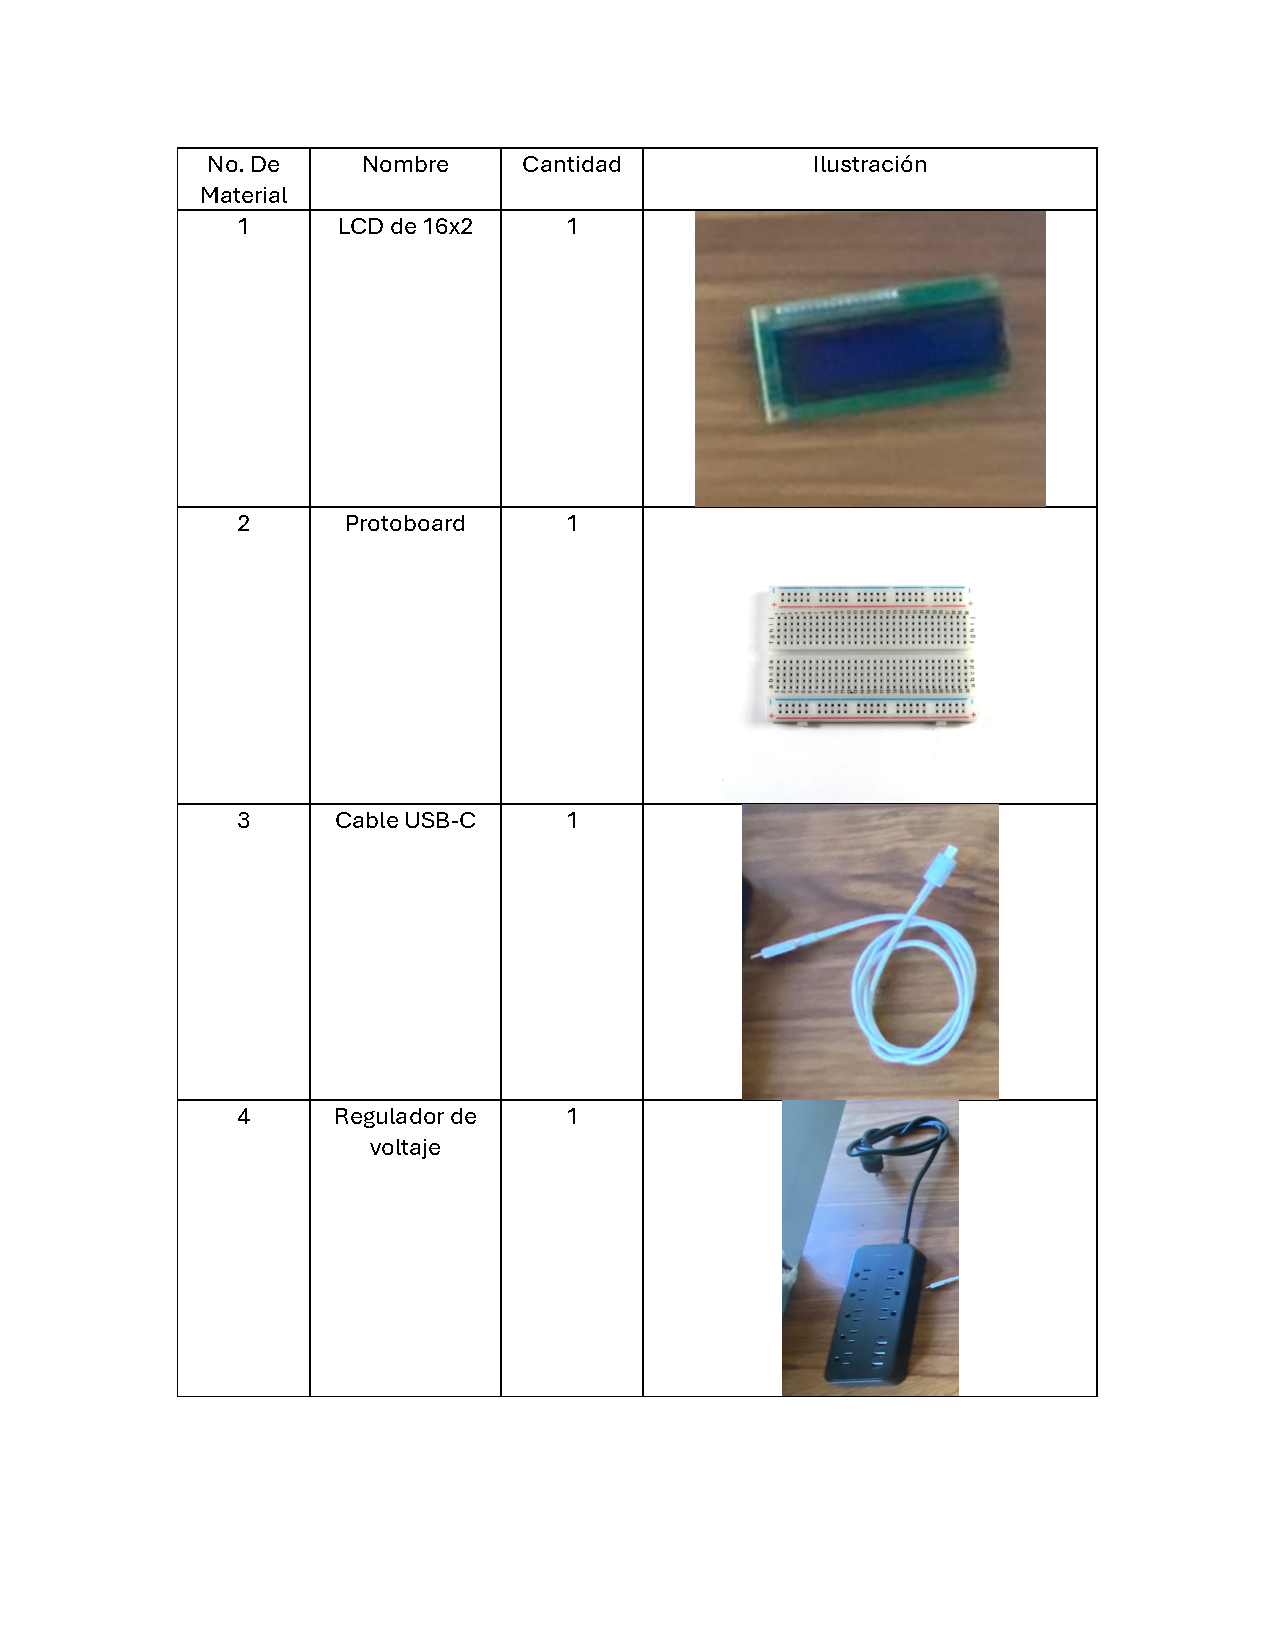
\includepdf[pages=-]{15/img/listaDeMateriales.pdf}
    \label{anexo:listaDeMateriales.pdf}

    \centering{\section[\appendixautorefname{}]{APÉNDICE}}
    \includepdf[pages=-]{15/img/manualDeEnsambleDeCircuitoElectronicoEsp32-c6.pdf}
    \label{anexo:manualDeEnsambleDeCircuitoElectronicoEsp32-c6.pdf}
    %%%%%%%%%%%%%%%%%%%%%%%%%%%%%%%%%%%%%%%%


\bibliographystyle{apalike}
\bibliography{15/referencias}

